\documentclass[11pt,spanish,a4paper]{article}
% Versión 1er cuat 2014 Víctor Bettachini < bettachini@df.uba.ar >

\usepackage{babel}
\addto\shorthandsspanish{\spanishdeactivate{~<>}}
\usepackage[utf8]{inputenc}
\usepackage{float}
\usepackage{units}
\usepackage{siunitx}
\usepackage{amsmath}
\usepackage{amstext}
\usepackage{amssymb}
\usepackage{graphicx}
\graphicspath{ {./graphs/} {../}}

\voffset-3.5cm
\hoffset-3cm
\setlength{\textwidth}{17.5cm}
\setlength{\textheight}{27cm}

\usepackage{lastpage}
\usepackage{fancyhdr}
\pagestyle{fancyplain}
\fancyhead{}
\fancyfoot{}
\fancyfoot[C]{ {\tiny Actualizado al \today} }
\fancyfoot[RO, LE]{Pág. \thepage/\pageref{LastPage}}
\renewcommand{\headrulewidth}{0pt}
\renewcommand{\footrulewidth}{0pt}


\begin{document}
\begin{center}
	\textsc{\large Física 2 (Físicos)} - Prof. Hernán Grecco\\
	\textsc{\large Primer Cuatrimestre - 2014}\\
	\textsc{\large Guía 3:}	Ecuación de ondas en una dimensión
\end{center}

\begin{enumerate}
\item Una cuerda de longitud \(L\) fija en sus extremos es lanzada a oscilar con igual amplitud en sus dos modos de menor frecuencia parte del repaso
	\begin{enumerate}
		\item Encuentre el apartamiento del equilibrio para cada punto de la cuerda en función del
			tiempo.
		\item ¿Con qué período se repite el movimiento?
		\item Grafíquelo para cuatro instantes equiespaciados dentro de un período.
	\end{enumerate}

\item Una cuerda de longitud \(L\) fija en un extremo y libre en el otro es lanzada a oscilar en sus modos 5 y 7 con igual amplitud, pero partiendo del reposo el modo 5 y de su máxima velocidad el modo 7.
	Repita los puntos del problema 1.

\item Mostrar que si \(\psi\) es solución de la ecuación de onda clásica, las funciones \(\phi_1\), \(\phi_2\) y \(\phi_3\)	definidas abajo también lo son.
	\[
		\phi_1 = \frac{\partial \psi}{\partial t} \qquad \phi_2 = \frac{\partial \psi}{\partial x} \qquad \phi_3 = \int\! \psi \mathrm{d}t
	\]

\item Se suelta una cuerda fija en sus extremos desde el estado inicial en reposo indicado en la figura.
	\begin{enumerate}
		\item calcule la evolución en el tiempo.
		\item ¿cuál es el modo excitado de mayor amplitud?
		\item ¿qué modos no son excitados?
	\end{enumerate}
	\begin{center}
		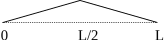
\includegraphics[width=0.3\linewidth]{g03e04}
	\end{center}

\item ¿Cómo cambia el problema anterior si el estado inicial es antisimétrico, como indica la figura?
	\begin{center}
		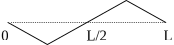
\includegraphics[width=0.3\linewidth]{g03e05}
	\end{center}

\item ¿Para qué valor de \(L_1\) se maximiza la excitación del segundo modo?
	¿Qué cambia musicalmente al cambiar \(L_1\)?
	\begin{center}
		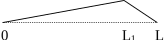
\includegraphics[width=0.3\linewidth]{g03e06}
	\end{center}

\item Se aplica una fuerza impulsiva sobre un 10\% del largo de una cuerda fija en sus extremos.
	El impulso es suficientemente rápido como para asumir que la cuerda no se movió apreciablemente durante su aplicación.
	\begin{enumerate}
		\item ¿Donde debe aplicarse el golpe para tener máxima amplitud en el quinto modo?
		\item ¿Y para tener máxima relación entre el quinto y el tercero?
	\end{enumerate}

\item Escriba la ecuación de onda para el caso del péndulo cuando la masa del hilo no es mucho menor que la del cuerpo suspendido.
	Para ello tenga en cuenta que la tensión varía a lo largo del hilo debido al peso del propio hilo.
	Muestre que las soluciones sinusoidales obtenidas para la cuerda ya no son solución.
	Discuta soluciones aproximadas.

\end{enumerate}
\end{document}
